% Format teze zasnovan je na paketu memoir
% http://tug.ctan.org/macros/latex/contrib/memoir/memman.pdf ili
% http://texdoc.net/texmf-dist/doc/latex/memoir/memman.pdf
% 
% Prilikom zadavanja klase memoir, navedenim opcijama se podešava 
% veličina slova (12pt) i jednostrano štampanje (oneside).
% Ove parametre možete menjati samo ako pravite nezvanične verzije
% mastera za privatnu upotrebu (na primer, u b5 varijanti ima smisla 
% smanjiti 
\documentclass[12pt,oneside]{memoir}

% Paket koji definiše sve specifičnosti mastera Matematičkog fakulteta
\usepackage{matfmaster}
\usepackage{minted}
\usemintedstyle{perldoc}
%
% Podrazumevano pismo je ćirilica.
%   Ako koristite pdflatex, a ne xetex, sav latinički tekst na srpskom jeziku
%   treba biti okružen sa \lat{...} ili \begin{latinica}...\end{latinica}.
%
% Opicija [latinica]:
%   ako želite da pišete latiniciom, dodajte opciju "latinica" tj.
%   prethodni paket uključite pomoću: \usepackage[latinica]{matfmaster}.
%   Ako koristite pdflatex, a ne xetex, sav ćirilički tekst treba biti
%   okružen sa \cir{...} ili \begin{cirilica}...\end{cirilica}.
%
% Opcija [biblatex]:
%   ako želite da koristite reference na više jezika i umesto paketa
%   bibtex da koristite BibLaTeX/Biber, dodajte opciju "biblatex" tj.
%   prethodni paket uključite pomoću: \usepackage[biblatex]{matfmaster}
%
% Opcija [b5paper]:
%   ako želite da napravite verziju teze u manjem (b5) formatu, navedite
%   opciju "b5paper", tj. prethodni paket uključite pomoću: 
%   \usepackage[b5paper]{matfmaster}. Tada ima smisla razmisliti o promeni
%   veličine slova (izmenom opcije 12pt na 11pt u \documentclass{memoir}).
%
% Naravno, opcije je moguće kombinovati.
% Npr. \usepackage[b5paper,biblatex]{matfmaster}

% Pomoćni paket koji generiše nasumičan tekst u kojem se javljaju sva slova
% azbuke (nema potrebe koristiti ovo u pravim disertacijama)
\usepackage{pangrami}

% Datoteka sa literaturom u BibTex tj. BibLaTeX/Biber formatu
\bib{matfmaster-primer}

% Ime kandidata na srpskom jeziku (u odabranom pismu)
\autor{Стефана Церовина}
% Naslov teze na srpskom jeziku (u odabranom pismu)
\naslov{Виртуелна машина Дартино- имплементација интерпретатора за платформу МИПС}
% Godina u kojoj je teza predana komisiji
\godina{2016}
% Ime i afilijacija mentora (u odabranom pismu)
\mentor{др Милена \textsc{Вујошевић Јаничић}\\ Универзитет у Београду, Математички факултет}
% Ime i afilijacija prvog člana komisije (u odabranom pismu)
\komisijaA{др Саша \textsc{Малков}\\ Универзитет у Београду, Математички факултет}
% Ime i afilijacija drugog člana komisije (u odabranom pismu)
\komisijaB{др Филип \textsc{Марић}\\ Универзитет у Београду, Математички факултет}
% Ime i afilijacija trećeg člana komisije (opciono)
% \komisijaC{}
% Ime i afilijacija četvrtog člana komisije (opciono)
% \komisijaD{}
% Datum odbrane (obrisati ili iskomentarisati narednu liniju ako datum odbrane nije poznat)
%\datumodbrane{}

% Apstrakt na srpskom jeziku (u odabranom pismu)
\apstr{%

}

% Ključne reči na srpskom jeziku (u odabranom pismu)
\kljucnereci{МИПС, систем са уграђеним рачунаром, интерпретатор,}

\begin{document}
% ==============================================================================
% Uvodni deo teze
\frontmatter
% ==============================================================================
% Naslovna strana
\naslovna
% Strana sa podacima o mentoru i članovima komisije
\komisija
% Strana sa posvetom (u odabranom pismu)
\posveta{Брату, мами и тати}
% Strana sa podacima o disertaciji na srpskom jeziku
\apstrakt
% Sadržaj teze
\tableofcontents*

% ==============================================================================
% Glavni deo teze
\mainmatter
% ==============================================================================

% ------------------------------------------------------------------------------
\chapter{Увод}
Појам "Интернет ствари" (енг. IOT- Internet of things) се све чешће среће, и он представља модел повезаности објеката који нас свакодневно окружују у огроман систем у оквиру ког међусобно комуницирају. Дефиниција "ствари" у оквиру појма "Интернет ствари" варира, али се може рећи да је то систем са уграђеним рачунаром(енг. embedded system) који преноси и прима информације путем мреже. Системи са уграђеним рачунаром су системи специјалне намене, који обављају једну или више функција које тој намени одговарају. Модерни системи са уграђеним рачунаром су углавном базирани на микроконтролерима, а ређе на микропроцесорима, зато што микроконтролере карактерише ефикасно управљање процесима у реалном времену, масовна производња, ниска цена и мала потрошња електричне енергије. Сматра се да је потенцијал за развој индустрије система са уграђеним рачунаром велики, и да је будућност у изградњи велики ИоТ система.\\

Писање апликација за системе са уграђеним рачунаром се обично своди на писање у програмском језику C, коришћење гцц(енг.GCC) или ллвм(енг. LLVM) компилатор, и коришћење неког алата за дебаговање, обично гдб(енг. gdb) који се налази на другом рачунару. Разлог због ког је окружење такво је то што микроконтролер садржи малу количину РАМ меморије, малу количину флеш меморије, па се на овако малом уређају не може покренути ниједан регуларни оперативни систем, а и микролинукс често захтева више РАМ меморије од оне којом микроконтролер располаже. Често се програмира у асемблерском језику. Због наведених услова, процес развоја апликација је доста успорен. 

Пошто се Веб апликације много брже развијају од апликација за системе са уграђеним рачунаром, дошло се на идеју да се омогући програмирање система са уграђеним рачунаром у вишем програмском језику Дарт, за који постоји подршка за развој Веб, серверских и мобилних апликација. Више о програмском језику Дарт биће речено у погрављу \ref{chp:dart}. Тако је настала виртуелна машина Дартино, са намером да се програмирање система са уграђеним рачунаром олакша и приближи што већем броју програмера. Дартино омогућава писање апликација за мале микроконтролере, на језику који доста личи на C, али је објектно-оријентисан и садржи разне погодности које процес имплементације доста олакшавају, те се апликације могу развијати брже и ефикасније. Ова виртуелна машина је детаљније описана у погрављу \ref{chp:dartino}.

У оквиру Дартино виртуелне машине биле су подржане само Интел и Арм архитектуре процесора. Због широке распрострањености МИПС процесора у системима са уграђеним рачунаром, развијен је интерпретатор за платформу МИПС, који је у међувремену званично интегрисан у Дартино пројекат. Имплементација интерпретатора описана је у поглављу \ref{chp:implementacija}, док се о платформи МИПС више може прочитати у поглављу \ref{chp:mips}.\\

% ------------------------------------------------------------------------------



% ------------------------------------------------------------------------------
\chapter{МИПС}
\label{chp:mips}
% ------------------------------------------------------------------------------

\section{ЦИСК и РИСК}

\section{Проточни систем (pipeline)}

\section{Специфичности МИПС платформе}

\section{Поређење МИПС платформе и Интел x86-64}

\section{Поређење МИПС платформе и АРМ}

\section{Архитектура МИПС32}

\section{Значај и употреба МИПС платформе у системима са уграђеним рачунаром}

% ------------------------------------------------------------------------------
\chapter{Програмски језик Дарт}
\label{chp:dart}
% ------------------------------------------------------------------------------

\section{Уопштено}

\section{Приватност}

\section{Конкурентност}

\section{Грешке и упозорења}

\section{Променљиве}

\section{Функције}

\section{Оператори}

\section{Класе}

\section{Интерфејси}

\section{Енумерације}

\section{Генерици}

\section{Уграђени типови}

\section{Библиотеке}

\section{Специфичности у односу на јаваскрипт}

\section{Платформе}


% ------------------------------------------------------------------------------
\chapter{Дартино}
\label{chp:dartino}
% ------------------------------------------------------------------------------
\section{Опис виртуелне машине}

Дартино виртуелна машина представља виртуелну машину за симулирање језика. Виртуелне машине за симулирање језика извршавају један програм, односно један процес. Имплементирају се са циљем обезбеђивања окружења за програме, независно од платформе, а имплементација се заснива на интерпретатору.

Као што је речено у уводу, Дартино виртуелна машина је настала са циљем да се писање апликација за микроконтролере олакша. Како би се направило боље окружење за рад, потребна је отворена и приступачна платформа, која ће већини програмера бити позната. Требало би омогућити статичку анализу кода, допуњавање кода, библиотеке са разним функционалностима, и тиме развијање апликација учинити ефикаснијим.

Пре Дартина је било могуће програмирати микропроцесоре у Дарту, али не и микроконтролере. Особине микроконтролера постављају велика додатна ограничења при развоју виртуелне машине која ће на њима радити. Обично се под виртуелном машином подразумева нешто што преводи изворни код у некакав међукод, и извршава га. Према томе, виртуелна машина садржи некакву компоненту за извршавање, сакупљач отпадака, омогућује препознавање класа и објеката, и има подршку за дебаговање.

Шта садржи Дартино виртуелна машина?
\begin{enumerate}
\item Компоненту за извршавање
\item Објектни модел
\item Сакупљач отпадака
\end{enumerate}

Ове три компоненте су неопходне када је у питању виши програмски језик као што је Дарт. Компилатор изворног кода је избачен, и направљен је систем у коме су компилатор и окружење за извршавање раздвојени, као што је случај код гцц-а или ллвм-а. Систем за дебаговање је да поједностављен и смањен.

Како су раздвојени компилатор и окружење за извршавање? Компилатор може да се налази било где, обично на рачунару где се развија апликација, и он комуницира са окружењем за извршавање које се потенцијално налази на другом систему. Интерфејс за комуникацију је једноставан, јер окружење за извршавање мора бити веома једноставно, како би одговарало карактеристикама миктроконтролера.
Окружење за извршавање садржи командни АПИ, преко ког му компилатор може затражити да уради одређене ствари. Испод тога се заправо налази стек машина, тако да се може поставити ново стање на стек окружења за извршавање, могу се правити класе, дефинисати објекти и методе путем овог АПИ-ја.

\begin{figure}[!ht]
  \centering
  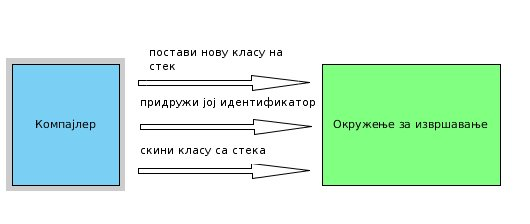
\includegraphics[width=0.8\textwidth]{compiler.jpg}
  \caption{Комуникација компилатора и окружења за извршавање}
  \label{fig:komunikacija}
\end{figure}

Како би компилатор знао где је која класа завршила у систему, и доделио им симболичка имена, омогућено му је да свакој класи придружи одређени идентификатор. Ови идентификатори окружењу за извршавање не значе ништа, али компилатор при примању објекта назад, зна да је инстанца одређене класе.
Сва комуникација се врши преко жичног протокола, тако да је омогућено удаљено извршавање, и обично је базирано на TCP/IP протоколу. На овај начин велики део посла се пребацује на компилатор, а окружење за извршавање се максимално упрошћава.

Шта се све може радити помоћу овог протокола? Најпре се може постављати структура програма, што обухвата:
\begin{enumerate}
\item Додавање нових класа на стек
\item Додавање нових метода на стек
\end{enumerate}
Може се мењати структура програма:
\begin{enumerate}
\item Мењање табела метода\\
Може се рећи "од овог тренутка желим да ова класа поред метода А има и метод Б". То значи да је омогућена висока интерактивност са системом.
\item Мењање шема\\
Мењање шема се односи на мењање класе, нпр.додавањем нових поља. Оно што се дешава у тој ситуацији је да се врши пролаз кроз све инстанце класе, и оне се ажурирају и прилагођавају новом формату класе.
\item Дебаговање
\begin{enumerate}
\item Покретање
\item Постављање зауставних тачака
\item Рестартовање
\end{enumerate}
\end{enumerate}
Систем за дебаговање једноставан и ограничен, јер не зна ништа о изворном коду.
\section{Модел програмирања}

Доњи слој чини традиционални оперативни систем са уграђеним рачунаром у реалном времену(нпр. Фри РТОС). Изнад тога се налази Дартино окружење за извршавање, које може извршавати више програма, независно, и они не морају знати ништа једни о другима. Ово се разликује од уобичајених система који раде на оперативном систему са уграђеним рачунаром, и који обично не могу да извршавају више независних компоненти, на независан начин. За сваки програм можемо имати више процеса, више инстанци програма, или делова програма, који се извршавају конкурентно.

\begin{figure}[!ht]
  \centering
  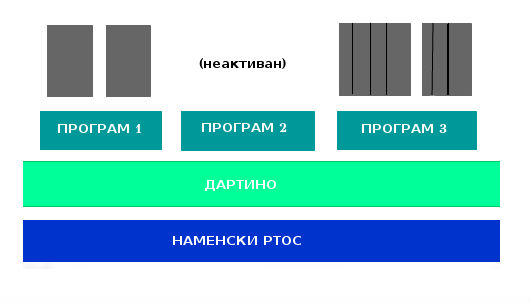
\includegraphics[width=0.7\textwidth]{arhitektura.jpg}
  \caption{Модел програмирања}
  \label{fig:model}
\end{figure}
На слици \ref{fig:model} је приказана ситуација када имамо 3 програма. Програм2 се тренутно не извршава, за Програм1 су покренуте две инстанце, док се Програм3  извршава у 7 нити.

\section{Значајне карактеристике}
\begin{enumerate} 
\item Лаки процеси

За сваки процес нам је потребно мало меморије, неколико стотина бајтова. Сав код и подаци у меморији се деле, па меморију заузимају само подаци који представљају процес. На овај начин ради већина оперативних система, али је то новина за оперативне системе са уграђеним рачунаром.

\item Блокирање процеса

Процес се може блокирати, при чему се не заузимају ресурси, већ се главна нит враћа систему. Разлог за то је што у системима са уграђеним рачунаром обично имамо мали фиксирани број нити, па не желимо да их блокирамо. 

\item Паралелизам

Уколико процесор има више језгара, процеси се могу извршавати паралелно.

\begin{minted}{javascript}
main() {
  for (int i = 0; i < 40000; i++) {
    Process.spawn(factoriel, 12);
  }
}

int factoriel(n) {
  if (n == 1) return 1;
  return n * factoriel(n-1);
}
\end{minted}
Могуће је покренути 40000 независних процеса, који ће бити лепо распоређени на одређени број језгара и извршавати се паралелно.

Како се могу користити процеси за манипулисање надолазећим конекцијама?

\begin{minted}{javascript}
var server = new ServerSocket("127.0.0.1", 0);
while(true) {
  server.spawnAccept((Socket socket){
	//izvrsava se u novom procesu
	socket.send(UTF.encode("Hello"));
	socket.close();
  })
}
\end{minted}

Креира се ServerSocket који представља сервер, затим се помоћу метода spawnAccept креира нови процес. У оквиру тог процеса се чека да клијент успостави конекцију са сервером, и самим тим блокира даље извршавање док се конекција не успостави. При успостављању конекције, клијент(socket) шаље серверу(server) поздравну поруку.


\item Комуникација

Комуникација између процеса се обавља слањем порука, помоћу канала и портова. Канал представља један ред порука. Порт представља могућност слања поруке каналу, и без приступа одеђеном порту, не може се слати порука каналу који чека на другој страни порта.

Блокирање слањем порука:

\begin{minted}{javascript}
final channel = new Channel();
final port = new Port(channel);
Process.spawn(() {
	int i=0;
	while(i < 50) {
		port.send(i++);
	}
});
while(true) {
	print(channel.receive());
}
\end{minted}
Један процес који шаље поруке, и функција print која блокира извршавање све док не прими следећу поруку.

\item Дељено непроменљиво стање између процеса
\begin{enumerate}
\item Сваки непроменљиви објекат се може слати као порука, без копирања
\item Више процеса могу користити исти објекат истовремено
\item Нема потребе за експлицитним примитивама за синхронизацију
\end{enumerate}

\item Изолате

Изолате су независни воркери, свака изолата има своју хип меморију, и за разлику од нити нема дељења меморије између изолата. Изолате комуницирају само преко порука. Могу се паузирати, наставити и убити.

\begin{minted}{javascript}
main() {
  Expect.equals(1597, fib(16));
  Expect.equals(4181, fib(18)); 
}

fib(n) {
  if (n <= 1) return 1;
  var n1 = Isolate.spawn(() => fib(n - 1));
  var n2 = Isolate.spawn(() => fib(n - 2));
  return n1.join() + n2.join();
}
\end{minted}
Пример употребе изолата за рачунање елемената Фибоначијевог низа, рекурзивно, покретањем две независне изолате.

\item Влакна

Влакна представљају нити извршавања у оквиру једног процеса, које деле спољну меморију, али не деле непроменљиву меморију. Омогућују да више независних нити једног процеса могу чекати на исту ствар(блокирати) независно једна од друге. На овај начин се имплементира вишеструка одвојена контрола тока.

\begin{minted}{javascript}
void publishOnChange(Socket socket, String propertyName, Channel input){
  int last = 0;
  while(true){
    int current = input.receive();
    if(current != last)
      socket.send(UTF.encode('("\$propertyName": \$current)'));
    last = current;
  
  }
}

Fiber.fork(() => publishOnChange(server, "temperature", temperatureSensor));
Fiber.fork(() => publishOnChange(server, "humidity", humiditySensor));

\end{minted}
Креирамо два влакна, у оквиру једног се чека на промену вредности у сензору за температуру, док се у оквиру другог чека на промену вредности у сензору за влажност ваздуха. Функција publishOnChange блокира извршавање док се у сензору за који је позвана не деси промена вредности. На овај начин је омогућено да се у оквиру једног процеса чека на више ствари, и нема паралелизма, већ се уколико дође до блокирања у једном влакну, прелази на извршавање следећег који је спреман за извршавање.

\item Корутине

Дартино има уграђену подршку за корутине. Корутине су објекти налик на функције, које могу давати више вредности, па су веома сличне генераторима. Када корутина врати вредност, зауставља се на тренутној позицији, а њен стек извршавања се чува за касније покретање. Када врати последњу вредност, сматра се завршеном, и више се не може покретати.

Пример употребе корутина:

\begin{minted}{javascript}
var co = new Coroutine((x) {
    Expect.isTrue(co.isRunning);
    Expect.equals(1, x);
    Expect.equals(2, Coroutine.yield(4));
    Expect.isTrue(co.isRunning);
});
Expect.isTrue(co.isSuspended);
Expect.equals(4, co(1));
Expect.isTrue(co.isSuspended);
Expect.isNull(co(2));
Expect.isTrue(co.isDone);
\end{minted}

\item Динамичко отпремање метода

Динамичко отпремање метода се односи на позивање преклопљених метода класа, при чему се проблем преклапања разрешава у фази превођења, а не у фази извршавања. Табела отпремања се имплементира као низ, у који се сваки метод, сваке класе, смешта на своју позицију. Позиција метода се рачуна помоћу редног броја класе и  позиције метода. Оно што је неопходно при добијању одређеног метода из табеле је провера да ли је резултат заправо оно што нам треба. Уколико није, значи да тражении метод одређене класе не постоји. Загарантовано је константно време отпремања, и табела отпремања се израчунава пре извршавања, па представља део апликације.
Пример прављења табеле отпремања:

\begin{minted}{javascript}
class A {
  metod1();
}

class B extends A {
  metod2();
}

class C extends B {
  metod1();
}

class D extends A {
  metod3();
}
\end{minted}

Класама редом придружимо бројеве: 0, 1, 2 и 3. Методима придружимо позиције на мало компликованији начин. Метод metod1, који је дефинисан у највећем броју класа, придружимо позицију 0, и он се смешта на почетак табеле. Методу metod2 придружимо позицију 3, и методу metod3 придружимо 4. Позиције морају бити јединствени бројеви, како не би дошло до преклапања метода. Приметимо да се могу појавити празне позиције у табели.

\begin{figure}[!ht]
  \centering
  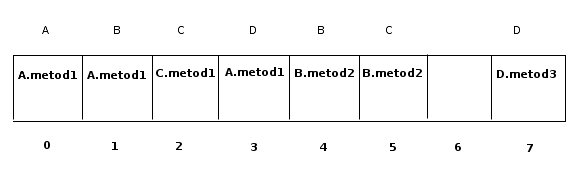
\includegraphics[width=0.7\textwidth]{otpremanje.jpg}
  \caption{Табела отпремања за дати пример}
  \label{fig:model}
\end{figure}


\end{enumerate}

\section{Најзначајније библиотеке}
\begin{enumerate}

\item file - АПИ за рад са датотекама. Подржано само када се Дартино извршава на ПОСИКС платформи.

\item ffi - 'foreign function interface' библиотека која омогућава да се из Дарт кода позивају функције дефинисане у неком другом програмском језику, нпр. функције програмског језика C.

\item http - Имплементација HTTP клијента.

\item mbedtls - TLS подршка, базирана на mbedtls. Ово се може користити на исти начин као нормални сокет (и да се прослеђује HTTP пакету).

\item mqtt - MQTT клијентска библиотека за MQTT протокол, IOT протокол за размену порука заснован на објављивању/претплати.

\item os - Приступ оператитивном систему. Подржано када се Дартино извршава на ПОСИКС платформи.

\item socket - Дартино имплементација TCP и UDP сокета

\item stm32 - Подршка за STM32 плоче.

\end{enumerate}

\section{Покретање Дарт програма помоћу Дартино ВМ}

Примарни начин за комуникацију са Дартино виртуелном машином је преко команде dartino. Ова команда комуницира са трајним(persistent) процесом, који ради сав тежи посао. Помоћу трајног процеса(dart) dartino компајлира програм, a помоћу Дартино виртуелне машине (dartino-vm) извршава и дебагује програме .\\

Нешто више о командама које се користе при покретању програма:
\begin{enumerate}
\item dartino\\
Ова команда је Ц++ програм. Намера је била да буде што једноставнији програм који једноставно прослеђује стандардне улазно/излазне сигнале трајном процесу преко сокета. Ово је мали извршни фајл за покретање компилатора. Компилатор је написан у Дарту и извршава се у оквиру Дарт виртуелне машине. 
\item dartino-vm \\
Самостална виртуелна машина која подржава превођење програма и покретање програма из бајткода.
\item dart \\
Трајни процес је Дарт програм: Класична Дарт виртуелна машина за покретање компилатора. Овај извршни фајл се не генерише у оквиру Дартина, већ је део Дарта. Трајни процес се састоји из главне нити, и неколико воркера. Главна нит ослушкује надолазеће конекције из дартино команде, и може да користи воркере да обави тражени задатак.
\end{enumerate}

Шта се заправо дешава када се покрене команда "dartino run hello.dart"? Дартино је подразумевано повезан на локалну сесију, која је повезана на локалну виртуелну машину која ради на нашем рачунару. "dartino" преводи код до бајткода, а онда га прослеђује "dartino-vm" која га извршава. Дартино виртуелна машина враћа резултат назад Дартину, и он га приказује.

Дартино подржава више сесија. Свака сесија може бити придружена различитој Дартино виртуелној машини, што омогућује кориснику да тестира више разлићитих уређаја истовремено. Тренутно је руковање сесијама експлицитно.

\begin{figure}[!ht]
  \centering
  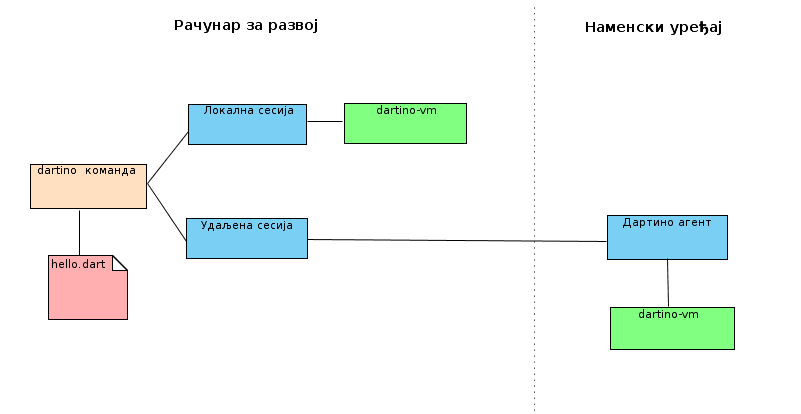
\includegraphics[width=0.9\textwidth]{sesije.png}
  \caption{Процес извршавања програма}
  \label{fig:izvrsavanje}
\end{figure}

Покретање програма у оквиру одређене сесије је омогућено на следећи начин: 

\begin{minted}{awk}
./out/DebugXMIPS/dartino create session my_session
\end{minted}
Креирање нове сесије "my\_session".

Након тога морамо да покренемо дартино виртуелну машину:
\begin{minted}{awk}
./out/DebugXMIPS/dartino-vm
\end{minted}
Након чега се исписује порука типа "Waiting for compiler on 127.0.0.1:61745". 61745 представља рандом генерисани порт.

У новом терминалу се прикачимо на дати сокет:
\begin{minted}{javascript}
./out/DebugXMIPS/dartino attach tcp_socket 127.0.0.1:61745 in session my_session
\end{minted} 

А затим покренемо жељени програм у оквиру те сесије:
\begin{minted}{awk}
./out/DebugXMIPS/dartino run hello.dart in session my_session
\end{minted}

Сесија се прекида помоћу следеће команде:
\begin{minted}{awk}
./out/DebugXMIPS/dartino x-end session my_session
\end{minted}


% ------------------------------------------------------------------------------
\chapter{Имплементација интерпретатора за платформу МИПС}
\label{chp:implementacija}
% ------------------------------------------------------------------------------

\section{Имплементација у програмском језику Ц++}


\section{Нумерички алгоритам у програмском језику Дарт}


% ------------------------------------------------------------------------------
\chapter{Закључак}
% ------------------------------------------------------------------------------


% ------------------------------------------------------------------------------
% Literatura
% ------------------------------------------------------------------------------
\literatura

% ==============================================================================
% Završni deo teze i prilozi
\backmatter
% ==============================================================================

% ------------------------------------------------------------------------------
% Biografija kandidata

% ------------------------------------------------------------------------------

\end{document} 
